\chapter{Mesh Shading} \label{cpt-mesh-shading}

% @TODO: Mention that this is rasterization pipeline!

Mesh Shaders were were first introduced to nVidia Touring \ac{GPU}s in 2018 as a part of
"a new programmable geometric shading pipeline" and build upon the compute programming 
pipeline \cite[Christoph Kubisch]{Kubisch2018}. Therefore, they aim to optimize work by 
using the available hardware more efficiently. This section breaks down the differences 
of the Mesh Shading Pipeline compared to the traditional Vertex Shading Pipeline. In order 
to evaluate these differences effectively, we start by having a closer look at the 
Vertex Shading Pipeline.

\section{The Vertex Shading Pipeline} \label{sec-vertex-shading-pipeline}

The term \emph{Vertex Shading Pipeline} refers to the traditional rendering pipeline, which 
describes the different steps of the creation of a final output image, generated by the 
computer. Central to this pipeline are two \ac{GPU} programs, called \emph{shaders}. The 
\emph{Vertex Shader} operates on the vertices of a given 3D model representation. 
The \emph{Pixel Shader} (also referred to as \emph{Fragment Shader}) operates on each pixel 
of the output frame buffer. Usually, the color values are calculated here, based on factors 
like light direction, camera position et cetera. \\

\begin{figure}[h]
    \centering
    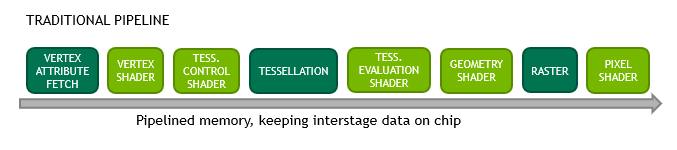
\includegraphics[width=\linewidth]{images/graphics/traditional-rendering-pipeline.png}
    \caption{The traditional rendering pipeline as presented by nVidia in \cite[Christoph Kubisch]{Kubisch2018}.}
    \label{fig:traditional-rendering-pipeline}
\end{figure}

\noindent
The traditional rendering pipeline consists of several fix, programmable and optional steps.
Figure \ref{fig:traditional-rendering-pipeline} shows these steps and their execution order. 
This pipeline represents more or less what the rendering pipeline has been for years up to this point. 
It is still used in most real time applications to this day, and even the mentioned Mesh Shading 
Pipeline relies on some of the central steps of this pipeline. To render a given scene, the relevant 
scene data is aggregated and passed to the \ac{GPU} for processing. For the purpose of this case study 
we are going to focus on the two main shader programs, as mentioned above. \\

% @TODO: Explain vertex data layout (indexed vertexlist) before! This is important for meshlets later!

\noindent
The \emph{Vertex Shader} takes the vertices of the given meshes in the scene as an input, aswell as 
some global and vertex specific data. The per-vertex data can include arbitrary data like color values, 
texture coordinates, transformations or the associated normal vector. The global data, which can be shared
by all the pipelines programs, can include data like a progressing time value or the position of the camera.
The vertex shader is called by the \emph{Input Assembler Stage} (called \emph{Vertex Attribute Fetch} in 
Figure \ref{fig:traditional-rendering-pipeline}) which implicitly invokes the vertex shader for each vertex 
of the mesh. This means that the computational cost increases with the amount of (visible) vertices in the scene. 
There are efforts to optimize the input data both on the \ac{CPU} and the \ac{GPU} which are addressed in section 
\ref{subsec-meshlet-occ-culling}.       % @TODO: Input chapter here


% @TODO: Explain every step of the pipeline ? 

% @TODO: Show input and output data of the Vertex Shader

% @TODO: What do I wanna say here?

% Good or even better to show evolution of rendering? -> Vertex Shaded Immediate Rendering -> 
% Vertex Shaded Deferred Rendering -> Mesh Shaded Deferred Rendering ? 

\section{The Mesh Shading Pipeline} \label{sec-mesh-shading-pipeline}

% @TODO: Mesh Shading Rendering Pipeline

\begin{figure}[h]
    \centering
    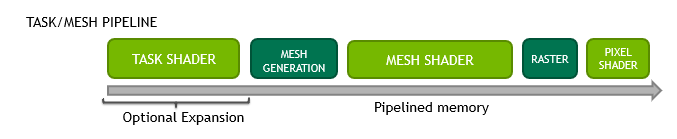
\includegraphics[width=\linewidth]{images/graphics/mesh-rendering-pipeline.png}
    \caption{The mesh shading pipeline as presented by nVidia in \cite[Christoph Kubisch]{Kubisch2018}.}
    \label{fig:mesh-rendering-pipeline}
\end{figure}

% @TODO: What are Mesh Shaders?


% @TODO: What are they good for?
% @TODO: How does the pipeline differ from the Vertex Shader Pipeline?

% @TODO: Meshlet Culling algorithm here or in 06_CaseStudy.tex?

\section{Differences and Comparison} \label{sec-differences-and-comparison}

- Differences and performance benefits

\subsection{Meshlet Occlusion Culling} \label{subsec-meshlet-occ-culling}

% @TODO: Meshlet Creation
